\PassOptionsToPackage{english}{babel}
\documentclass{wissdoc}
%\documentclass[oneside]{wissdoc}
% ----------------------------------------------------------------
% Diplomarbeit - Hauptdokument
% ----------------------------------------------------------------
% wissdoc Optionen: draft, relaxed, pdf, oneside --> siehe wissdoc.cls
% ------------------------------------------------------------------


% Packages für Deckblatt
\usepackage[absolute]{textpos} 	%Textboxen an absolute Position setzen
\usepackage{setspace}						%Zeilenabstand anpassen
\usepackage{color}							%Farbige Schrift
\usepackage{graphicx}						%Einbinden von Grafiken

% Weitere packages: (Dokumentation dazu durch "latex <package>.dtx")
% \usepackage{varioref}
% \usepackage{verbatim}
% \usepackage{float}    %z.B. \floatstyle{ruled}\restylefloat{figure}
%\usepackage{subfig}
\usepackage{wrapfig}
\usepackage{subfigure}
\usepackage[english,ngerman]{babel}

\usepackage[T1]{fontenc}
\usepackage[ansinew]{inputenc}

% Refernziere Kapiteln
\usepackage{hyperref}

% Zitaten
\usepackage[]{dirtytalk}
%\usepackage{epigraph}

% Footnote
\usepackage{scrextend}

% Math
\usepackage{amsmath}

% Zeilenabstand nach Vorgabe - Falls gefordert
%\setstretch{1,3} 

% Inhaltsangabe auf Unterabschnitte(2 Ebenen) begrenzen
\setcounter{tocdepth}{2}


% \usepackage{color}    % Farbiger/grauer Text
% \usepackage{colortbl}   % Farbige/graue Tabellenzeilen und -spalten!! <--
% \usepackage{fancybox} % für schattierte,ovale Boxen etc.
% \usepackage{tabularx} % automatische Spaltenbreite
% \usepackage{supertab} % mehrseitige Tabellen
%% ---------------- end of usepackages -------------

%% Informationen für die PDF-Datei
\hypersetup{pdfauthor={Max Mustermann},%
            pdftitle={Bachelorarbeit},%
            pdfsubject={Titel der Arbeit},%
            pdfkeywords={Forschung, Entwicklung, Funktechnik},%
            pdfproducer={LaTeX},%
            pdfcreator={pdfLaTeX}
}

% Macros, nicht unbedingt notwendig
%%%%%%%%%%%%%%%%%%%%%%%%%%%%%%%%%%%%%%%%%%%%%%%%%%%%%%%%%%
% macros.tex -- einige mehr oder weniger nuetzliche Makros
%%%%%%%%%%%%%%%%%%%%%%%%%%%%%%%%%%%%%%%%%%%%%%%%%%%%%%%%%%


%%%%%%%%%%%%%%%%%%%%%%%
% Kommentare 
%%%%%%%%%%%%%%%%%%%%%%%
\ifnotdraftelse{
\newcommand{\Kommentar}[1]{}
}{\newcommand{\Kommentar}[1]{{\em #1}}}
% Alles innerhalb von \Hide{} oder \ignore{} 
% wird von LaTeX komplett ignoriert (wie ein Kommentar)
\newcommand{\Hide}[1]{}
\let\ignore\Hide

%%%%%%%%%%%%%%%%%%%%%%%%%
% Leere Seite ohne Seitennummer, wird aber gezaehlt
%%%%%%%%%%%%%%%%%%%%%%%%%

\newcommand{\leereseite}{% Leerseite ohne Seitennummer, n�chste Seite rechts (wenn 2-seitig)
 \clearpage{\pagestyle{empty}\cleardoublepage}
}

%%%%%%%%%%%%%%%%%%%%%%%%%%
% Neue Seite rechts, leere linke Seite ohne Headings
%%%%%%%%%%%%%%%%%%%%%%%%%%
\newcommand{\xcleardoublepage}
{{\pagestyle{empty}\cleardoublepage}}

%%%%%%%%%%%%%%%%%%%%%%%%%%
% Tabellenspaltentypen (benoetigt colortbl)
%%%%%%%%%%%%%%%%%%%%%%%%%%
\newcommand{\PBS}[1]{\let\temp=\\#1\let\\=\temp}
\newcolumntype{y}{>{\PBS{\raggedright\hspace{0pt}}}p{1.35cm}}
\newcolumntype{z}{>{\PBS{\raggedright\hspace{0pt}}}p{2.5cm}}
\newcolumntype{q}{>{\PBS{\raggedright\hspace{0pt}}}p{6.5cm}}
\newcolumntype{g}{>{\columncolor[gray]{0.8}}c} % Grau
\newcolumntype{G}{>{\columncolor[gray]{0.9}}c} % helleres Grau

%%%%%%%%%%%%%%%%%%%%%%%%%%
% Anf�hrungszeichen oben und unten
%%%%%%%%%%%%%%%%%%%%%%%%%%
\newcommand{\anf}[1]{"`{#1}"'}

%%%%%%%%%%%%%%%%%%%%%%%%%%
% Tiefstellen von Text
%%%%%%%%%%%%%%%%%%%%%%%%%%
% S\tl{0} setzt die 0 unter das S (ohne Mathemodus!)
% zum Hochstellen gibt es uebrigens \textsuperscript
\makeatletter
\DeclareRobustCommand*\textlowerscript[1]{%
  \@textlowerscript{\selectfont#1}}
\def\@textlowerscript#1{%
  {\m@th\ensuremath{_{\mbox{\fontsize\sf@size\z@#1}}}}}
\let\tl\textlowerscript
\let\ts\textsuperscript
\makeatother

%%%%%%%%%%%%%%%%%%%%%%%%%%
% Gau�-Klammern
%%%%%%%%%%%%%%%%%%%%%%%%%%
\newcommand{\ceil}[1]{\lceil{#1}\rceil}
\newcommand{\floor}[1]{\lfloor{#1}\rfloor}

%%%%%%%%%%%%%%%%%%%%%%%%%%
% Average Operator (analog zu min, max)
%%%%%%%%%%%%%%%%%%%%%%%%%%
\def\avg{\mathop{\mathgroup\symoperators avg}}

%%%%%%%%%%%%%%%%%%%%%%%%%%
% Wortabk�rzungen
%%%%%%%%%%%%%%%%%%%%%%%%%%
\def\zB{z.\,B.\ }
\def\dh{d.\,h.\ }
\def\ua{u.\,a.\ }
\def\su{s.\,u.\ }
\newcommand{\bzw}{bzw.\ }

%%%%%%%%%%%%%%%%%%%%%%%%%%%%%%%%%%%
% Einbinden von Graphiken
%%%%%%%%%%%%%%%%%%%%%%%%%%%%%%%%%%%
% global scaling factor
\def\gsf{0.9}
%% Graphik, 
%% 3 Argumente: Datei, Label, Unterschrift
\newcommand{\Abbildung}[3]{%
\begin{figure}[tbh] %
\centerline{\scalebox{\gsf}{\includegraphics*{#1}}} %
\caption{#3} %
\label{#2} %
\end{figure} %
}
\let\Abb\Abbildung
%% Abbps
%% Graphik, skaliert, Angabe der Position
%% 5 Argumente: Position, Breite (0 bis 1.0), Datei, Label, Unterschrift
\newcommand{\Abbildungps}[5]{%
\begin{figure}[#1]%
\begin{center}
\scalebox{\gsf}{\includegraphics*[width=#2\textwidth]{#3}}%
\caption{#5}%
\label{#4}%
\end{center}
\end{figure}%
}
\let\Abbps\Abbildungps
%% Graphik, Angabe der Position, frei w�hlbares Argument f�r includegraphics
%% 5 Argumente: Position, Optionen, Datei, Label, Unterschrift
\newcommand{\Abbildungpf}[5]{%
\begin{figure}[#1]%
\begin{center}
\scalebox{\gsf}{\includegraphics*[#2]{#3}}%
\caption{#5}%
\label{#4}%
\end{center}
\end{figure}%
}
\let\Abbpf\Abbildungpf

%%
% Anmerkung: \resizebox{x}{y}{box} skaliert die box auf Breite x und H�he y,
%            ist x oder y ein !, dann wird das uspr�ngliche 
%            Seitenverh�ltnis beibehalten.
%            \rescalebox funktioniert �hnlich, nur das dort ein Faktor
%            statt einer Dimension angegeben wird.
%%
% \Abbps{Position}{Breite in Bruchteilen der Textbreite}{Dateiname}{Label}{Bildunterschrift}
%

\newcommand{\refAbb}[1]{%
s.~Abbildung \ref{#1}}

%%%%%%%%%%%%%%%%%%%%
%% end of macros.tex
%%%%%%%%%%%%%%%%%%%%

% Print URLs not in Typewriter Font
\def\UrlFont{\rm}

\newcommand{\blankpage}{% Leerseite ohne Seitennummer, nächste Seite rechts
 \clearpage{\pagestyle{empty}\cleardoublepage}
}

%% Einstellungen für das gesamte Dokument

% Trennhilfen
% Wichtig!
% Im german-paket sind zusätzlich folgende Trennhinweise enthalten:
% "- = zusätzliche Trennstelle
% "| = Vermeidung von Ligaturen und mögliche Trennung (bsp: Schaf"|fell)
% "~ = Bindestrich an dem keine Trennung erlaubt ist (bsp: bergauf und "~ab)
% "= = Bindestrich bei dem Worte vor und dahinter getrennt werden dürfen
% "" = Trennstelle ohne Erzeugung eines Trennstrichs (bsp: und/""oder)

% Trennhinweise fuer Woerter hier beschreiben
\hyphenation{
% Pro-to-koll-in-stan-zen
% Ma-na-ge-ment  Netz-werk-ele-men-ten
% Netz-werk Netz-werk-re-ser-vie-rung
% Netz-werk-adap-ter Fein-ju-stier-ung
% Da-ten-strom-spe-zi-fi-ka-tion Pa-ket-rumpf
% Kon-troll-in-stanz
}

%Tabellen Kommandos
\newcolumntype{L}[1]{>{\raggedright\arraybackslash}p{#1}}
\newcolumntype{C}[1]{>{\centering\arraybackslash}p{#1}}
\newcolumntype{R}[1]{>{\raggedleft\arraybackslash}p{#1}}

% Index-Datei öffnen
\ifnotdraft{\makeindex}
%%%%%%%%%%%%%% includeonly %%%%%%%%%%%%%%%%%%%
% Es werden nur die Teile eingebunden, die hier aufgefuehrt sind!
%\includeonly{%
%titelseite,%
%erklaerung,%
%kurzfassung,%
%einleitung,%
%analyse,%
%entwurf,%
%implemen,%
%zusammenf%
%}
%%%%%%%%%%%%%%%%%%%%%%%%%%%%%%%%%%%%%%%%%%%%%%
\begin{document}
\selectlanguage{english}
%Auskommentiert, da nicht notwendig für das Praktikum
%\ifnotdraft{
	%%%%Vorlage
	%%% Deckblatt - Hochschule Augsburg
%%%Deckblatt

\textblockorigin{20mm}{30mm}

\thispagestyle{empty}\null
%%%%Logo - Hochschule Augsburg - Informatik
\begin{textblock}{10}(8.0,1.1)
\begin{figure}[h]
	\centering
		
\includegraphics[width=0.45\textwidth]{logos/hsa_informatik_logo_lq.pdf}
\end{figure}

\end{textblock}

%%% Text unter Logo
\begin{textblock}{15}(12.43,2.1)
	\LARGE
	\textsf{
		\textbf{\textcolor[rgb]{1,0.41,0.13}{\\
			\begin{flushleft}
				Faculty of\\
				Informatics\\
			\end{flushleft}
			}
		}
	}
\end{textblock}

%%%%Textbox links - Informationen
\begin{textblock}{15}(2,1.4)
	%\LARGE
	\begin{flushleft}
		\begin{spacing} {1.2}
			\huge	
				\textbf{Bachelor Thesis}
				\vspace{30pt}
				\\
				%\textcolor[rgb]{1,0.41,0.13}{\\
				%\textbf{Bachelorarbit}}\\
				\vspace{60pt}
			\LARGE
				Field of study\\
				Technische Informatik\\
				\vspace{30pt}
				Florian P�rvu\\
				\vspace{60pt}		
				Thesis Title:	C++ Crossplatform Bibliothek zur Performanceanalyse\\ \hspace{31mm}von Anwedungen unter dynamisch generierten Lasten\\
				\vspace{60pt}		
			\LARGE
				First examiner: Prof. Dr. Thomas Kirchmeier\\
				Second examiner: Prof. Dr. Hubert H�gl\\
				\vspace{10pt}		
				Submission date: 20.01.2022\\
			\end{spacing}
		\end{flushleft}
		
\end{textblock}



%%%%Textbox rechts - Hochschule
\begin{textblock}{5}(12.45,9.0)
	\scriptsize
	\textcolor[rgb]{1,0,0}{\\
		\begin{flushleft}
			\begin{spacing} {1.3}
				Hochschule f\"ur angewandte\\
				Wissenschaften Augsburg\\
				\vspace{4pt}
				An der Hochschule 1\\
				D-86161 Augsburg\\
				\vspace{4pt}
				Tel\hspace{2pt} +49 821 55 86-0\\
				Fax +49 821 55 86-3222\\
				www.hs-augsburg.de\\
				info(at)hs-augsburg-de
			\end{spacing}
		\end{flushleft}
		}
\end{textblock}


%%%%Textbox rechts unten - Fakult�t und Autor
\begin{textblock}{5}(12.45,11.5)
	\scriptsize
		\begin{flushleft}
			\begin{spacing} {1.3}
				Faculty of Informatics\\
				Tel \hspace{12pt} +49 821 55 86-3450\\
				Fax \hspace{10pt} +49 821 55 86-3499\\
				\vspace{6pt}
				Bachelor Thesis author\\
				Florian P�rvu\\
				Asternweg 2\\
				86399 Bobingen\\
				Tel +49 176 3693 7974\\
				pflorian306@gmail.com\underline{}\\
			\end{spacing}
		\end{flushleft}
	\end{textblock}
\pagebreak  %<-- Nach Vorgabe der HS Augsburg
	%
	%%%% Innere Titelseite 
 	%\include{titelseite} %<-- Vorgabe Prüfer oder frei wählbar
	%
	%%%%Optional - Falls von der Firma gefordert
	%\include{sperrvermerk}
	%
	%%%%Pflicht
 	%\include{erklaerung}
	%
	%%% Leere Seite bei zweiseitigem Druck
	%\ifnotonesideelse{\blankpage}{}
	%\include{kurzfassung}
	%%% Leere Seite bei zweiseitigem Druck
	%\ifnotonesideelse{\blankpage}{}
%}



%
%% ++++++++++++++++++++++++++++++++++++++++++
%% Verzeichnisse
%% ++++++++++++++++++++++++++++++++++++++++++
\pagenumbering{roman}
\ifnotdraft{
\tableofcontents
% Leere Seite bei zweiseitigem Druck
\ifnotonesideelse{\blankpage}{}
%\listoffigures
%% Leere Seite bei zweiseitigem Druck
%\ifnotonesideelse{\blankpage}{}
%\listoftables
%% Leere Seite bei zweiseitigem Druck
%\ifnotonesideelse{\blankpage}{}
}
%% ++++++++++++++++++++++++++++++++++++++++++
%% Hauptteil
%% ++++++++++++++++++++++++++++++++++++++++++
\graphicspath{{figures/}}
\pagenumbering{arabic}

%%% Ab hier eigene Kapitel einfügen
%%% Kapitel sind analog zur Wordvorlage zu wählen
%Einleitung.tex
%
\chapter{Introduction}
\section{Motivation}
\subsection{Choosing the right tools}
When the computer was first invented, the world was much simpler and at the same time much rougher. The computers back then understood only a limited number of instructions and the tools that one needed to learn in order to conquer these new machines were unsophisticated (regarding the today's standard). At the same time people were restrained by the small size of memory and the lack of freedom when it came to working with computers. Back in the days, a typical computer was for example the \textit{Compaq Presario 425}, which had a 25MHz Intel 486 CPU (so it could execute 25 000 000 instructions per second) and 200MiB hard disk\cite{snowden}\footnote{For users not familiar with memory, as of April 2021, the size of the game \textit{Call of Duty: Modern Warfare} is around 230GiB. That is circa 1000 times bigger than the hard drive of \textit{Compaq Presario 425}}. As time passed engineers around the world worked together and upgraded the gadget and each year they increased the number of commands and the memory of computers and so created the machine to what it is today known as a \textit{personal computer}(short PC).
The new sets of instructions were also made differently in order to satisfy distinctive needs and in time they developed themselves into programming languages known today.\\
Despite the numerous amount of languages, not all of them are used.
A study made in 2020 researched 50 projects of an open source project management platform called \textit{Gitee}, showing which programming language is likely to be more popular based on multiple factors such as the popularity and attention the projects were getting on the platform. The results were split in five categorizes as showing in fig. \ref{programming_popularity}.
As observed the languages that maintain their popularity over the time are C\#, Java, C++, Python and JavaScript\cite{9434501}.
\begin{figure}[!htbp]
	\centering
	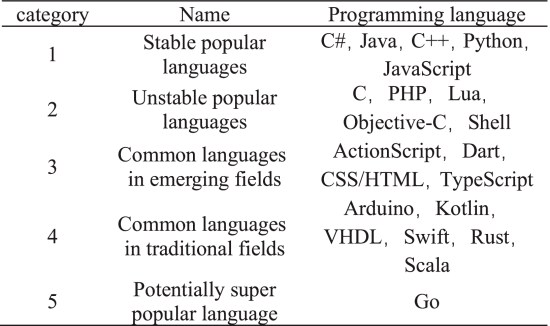
\includegraphics[width=0.60\textwidth]{../figures/einleitung/programming_popularity.png}
	\caption{Classification Results of Programming Languages}
	\label{programming_popularity}
\end{figure}\\
Showing this fact one could wonder, why even bother using the complicated C++, when there are other more easier options like Java or Python. The answer to this question can be read in the title of this thesis. It comes to performance.\\
A paper published in 2006 stated that when it came to performance such as memory for example, C++ was far superior in comparison to Java. It was mentioned that modern languages like Java or C\# hide their complexity under the hood. To prove this statement the author coded himself \dq a program that manipulated half a billion objects. Its C++ implementation required 3 Gbytes of real memory to run. A Java implementation would easily need that amount of memory just to store the objects'housekeeping data\dq{}. He also added that the language, although complicated with its huge size and complexity, comes as a combination of \dq extreme efficiency and expressiveness\dq{}. Nevertheless it was mentioned that for smaller devices such as an MCU\footnote{Microcontroller Unit} or systems code, using the C language is the way to go\cite{1657941}.\\
This lead me to the conclusion, that in order to still have a newer interface using OOP\footnote{Object Oriented Programming} and at the same time compatibility with the efficient C language, in which many operating systems are coded, C++ is the best candidate of them all. However performance is a vague term and can describe a lot of things, that's why, to better understand my vision, one should get a glimpse of my own understanding about \textit{Performance} 
\subsection{Performance \& Testing}
Performance of software is the process of analyzing a given program and reacting to problems that may or may not occur during runtime. The less unexpected problems emerge, the better the performance of that software\cite{8432081}. 
To make sure fewer problems occur, one could adopt methods like the \textit{Software Performance Engineering}, which uses quantitative techniques to identify designs with lesser flaws and so spare the developers significant time in their implementation\cite{4299916}. An idealistic scenario would be, if the product would have no flaws at all. But as many know, perfectness is hard to achieve, even harder if people keep developing the product. Even if the outcome may be perfect at a certain point in time, the continuous development will certainly show incompatibilities with the functional state of the product.
\begin{center}
	\say{If anything can go wrong, it will}
	\begin{flushright}
		\textit{Murphy's law}
	\end{flushright}
\end{center}
To avoid the release of a defect product and support the \textit{SPE} approach, one needs to implement additional tests, because bugs can appear even after deployment as the development process advances.\\
Testing in the IT-Branch is an approach with the main goal of finding bugs in a software program or application. These bugs refer to errors or faults and can occur because of a bad commands sequence specified in the program's source code or incompatibility of other member of the program. This can often occur especially when the \dq amount of libraries are high and the mutual dependencies complex\dq{}\cite{7302456}. A successful test can be achieved when its main requirements are met. Some examples would be the execution on different environments, time constraints or delivering expected outputs for randomly chosen inputs. Conditions are set by the tester and may vary. These are frequently chosen based on user cases and logical expectations.
\subsection{General}
Most companies put a lot of effort in delivering high performance products to their customers. In order to do so, each of them test their gadgets, machines or software for possible failure scenarios. The test phases usually take place before the release of a new product or the deployment of an update that brings new features to an existing product.\\
Now-a-days tests are being fully automated, which decreases the failure possibility that can happen because of human errors\cite{8389562}. Unfortunately the creation of fully automated tests is not as easy as it may sound. Many testing developers know the struggle of finding the right tools for the job without filling their projects with unnecessary dependencies that will overload the program and occupy valuable memory.
\begin{center}
	\say{As ironic as it seems, the challenge of a tester is to test as little as possible. Test less, but test smarter}
	\begin{flushright}
		\textit{Federico Teldo, Co-Founder Abstracta US}
	\end{flushright}
\end{center}
Additionally the problem enhances when a company reaches a certain size with a significant number of customers, which tend to run the product on different machines and architectures. In order to keep their customers, producers need to adapt their products to support newer or older machines. This makes software analysis even more difficult because of the increasing complexity, which comes with different systems. For this reason many companies dedicated themselves to creating programs that focus only on software examination and fixing bugs that may occur during an analysis	. In time a new trend has been created with demands so high that rapidly developed itself into a new market section.\\
\section{Growing markets}
For the last decade the software testing market has been developing and now it has grown so big that it would be foolish to ignore it. According to \dq Global Market Insights\dq{} the testing software market has grown up to 40 billion dollars by the end of 2020 and is predicted to grow up to 60 billion dollars in the next 6 years.\cite{GMI}\\
\textit{\dq People may lie, but number don't\dq}. Multiple scientific papers and studies enforce this statement with different statistics of industries, which started adapting and reacting to this trend using the model \dq EaaS\dq{} which stands for \textit{Everything as a service} and created \textit{ Testing as a Service}(TaaS). With this model customers not only pay for the current state of a product, but also for a service subscription, where they get updates and new features for the specific product and additional support from the company. The advantages that benefit the customer are set by the company for each of their subscription. (The basic rule is that you get more accurate results if you pay more). This service usually targets three groups: Developers, End Users and Certification Services.\cite{10.1145/1807128.1807153}. With the growing popularity of these services, companies quickly got blind sided by the convenience of paying less for experts with system knowledge and having them create software specific tests. In reality they would get disappointed by the advantages and cost comparison of putting in the effort to create testing methods specific for their own products. 
\begin{figure}[!htbp]
	\centering
	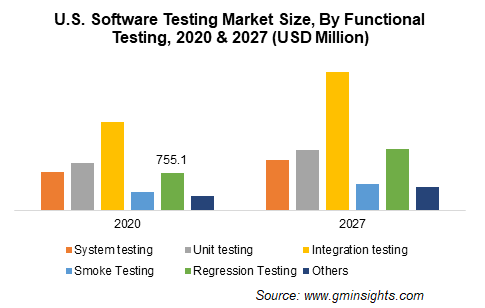
\includegraphics[width=0.80\textwidth]{../figures/einleitung/US_marketsize.png}
	\caption{US Software Market Size\cite{GMI}}
	\label{US_marketsize_graph}
\end{figure}

\subsection{The costs of perfection}
\label{costs}
Firms often tend to overlook costs of testing tasks that are insignificant in comparison to the total price of the project. However if these costs are reoccuring, their total price can go up to 40\% of the total project's costs\cite{8822082}.\\
There are two common ways to cope with this problem. First, one could use a third party software that specializes in testing other companies's software. This has its advantages, because the tests are already written to work on most compilers for a majority of programming languages and the continuous support and development through customer feedback. The bad part though, is the pricing, which may or may not be a problem for a company (depending on its size), the code's ownership and additional privacy issues, because we can't look behind the curtains of a compiled software, therefore we cannot tell what kind of data the program stores about the user or whom may it send it to.\\
The second way it would be to let the company's developers test themselves. This method proves often quite efficient, because they are the ones who programmed the software, therefore the best candidates to repair possible bugs and the company is not exposed to any additional privacy risks. However the whole process needs to be led by someone experienced enough to correctly organize current tasks, but also future ones. the staff management and avoid expensive commitments such as time and budget. At the begging, in house development may be even more expensive than buying a testing software, but in the long run it will be cheaper as the testing process gets more and more refined.\\
It was proven that the cost of finding an error is about \$50 on average \cite{10.1145/1010773.1010774}, and is said that fixing an error after the software was released is four times more expensive than compared to if it was found during the testing phase\cite{10.1007/978-981-10-8848-3_46}. That amount of money covers not only for direct testing, which includes the staff, system and program testing, resources, computer time, etc. , but also for indirect testing, which refers to actions that take place because of poor direct testing, like rewriting code, additional analysis meetings or debugging. To avoid these financial expenses, companies can train their developers to consider failure scenarios of the product early in the development stage.

\subsection{Common approaches}
In order to deliver a defect-free product, managers create testing strategies.
To develop the most suitable strategy, they must identify the key components for it. These can be identified mostly by answering the following questions adapted from \cite{10.1007/978-981-10-8848-3_46}:
\begin{enumerate}
	\item Is the objective clear specified?
	\item What tools will be used?
	\item Is the system fully/partially automated?
	\item How will the test benefit the project?
\end{enumerate}
Additionally, the results and procedures need to be recorded in order to make testing phases smoother, because the same errors may occur in the future.
% enumarate:
% weitere heruasforderung - unterschiedliche OS mit teilweise spezifischen testanforderungen
% diese äußern sich vor allem im Perfromancebetrachtungen -> zusätzliche Aufwände und Herausforderungen
% wenn das profitable ist, dann sollte das auf alle OS laufbar sein um den ganzen Markt zu erreichen
% bedarf eines Tools das auf alle OS anwendbar ist und vergleichbare Ergebnisse zeigt
% 
\section{Benchmarking}
In addition to testing, companies also have the desire to reach as many customers as possible. In order to do that many tend to create benchmarks that show the product's superiority in comparison to other products that fulfill the same task and reduce production costs.\\
According to the \textit{Standard Performance Evaluation Corporation} (short \textit{SPEC}), a benchmark is a \dq test, or set of tests, designed to compare the performance of one computer system against the performance of others\dq{}\cite{spec-benchmark}. A method developed by \textit{Infineon Technologies AG} ,written by Lukas Klaus, explains \dq The intention [...] [to] keep cost of test constant relative to overall cost of goods sold\dq{}. Klaus mention that once the yearly costs of production were established, once can come up with a financial plan that compares the manufacturing expenses with the \dq hypothetical best case if all products in question were at benchmark performance\dq{}. The method can additionally create in an indicator, which can be calculated by dividing test costs by the revenue of sold goods\cite{4221595}. This can be used to help decisions on which part is worth improving in order to create the best product while maximizing customer satisfaction.\\  
This leads to the question \dq What makes a good benchmark?\dq{}.\\
A paper written by Maya Daneva of Institute of Business Information Systems at the University Of Saarland answered this explaining the designs and usage of software benchmarking. According to her the targets of this approach can be classified in different classes of organizations with different set of goals. The most relevant for this thesis are software developers, distributors, testing laboratories and researchers, as well as certifications offices, academic intuitions and independent benchmarking companies. For a well made benchmark, Daneva introduced six crucial criterias\cite{Daneva1995}:
\begin{enumerate}
	\item Pertinence 
	\item Functional coverage   
	\item Understandability 
	\item Ease of use  
	\item Interpretability
	\item Reproducibility
\end{enumerate}    
When creating the benchmark one would try to achieve perfectness in every aspect of each criteria, but the reality often tends to disappoint our expectations. To explain this in detail you could think about these criteria as a hexagon with six angles. When the developer tries to implement one side of the hexagon to perfection he often would have to give up on other sides as pictured in Figure \ref{hexagon_criterias}. Most of the times one needs to identify the most important aspect that matters the most to him and choose it over less relevant ones (though this doesn't have to be always the case)
\begin{figure}[htbp]
	\centering
	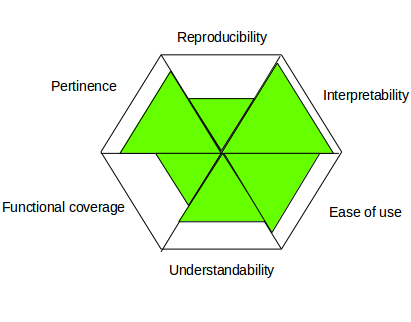
\includegraphics[width=0.6\textwidth]{../figures/einleitung/hexagon.png}
	\caption{Hexagon of criteria}
	\label{hexagon_criterias}
\end{figure}
\\In order to generate reliable statistics, the creator also needs to considerate the additional workload the benchmark is creating and to differentiate between the actual strains put on the system by the application at hand and those created by the benchmark. 
\subsection{Workload}
The definition for workload varies from field to field. In the IT-branch it is defined as a unit of measure for your CPU (mostly in \%). This tells the user how well his system can handle the number of current running processes.\\
Workloads are made out of two parts: the executable part and the non-executable part. The executable part refers to code that is being executed when an application software is being executed. The non-executable part refers to the workload produced in order for the executable part to have \dq a well-defined and reproducible manner\dq{}. One can also differentiate between natural and artificial workload. Natural workloads are produced by software executing useful tasks and benchmarks that deliver statistics based on such workloads are also called \textit{natural benchmarks}. Artificial workloads however are generated by code that tries to mimic real workload (most time irrelevant code like the incrementation of a variable in a loop). Most benchmarks often implement artificial workloads ,because they \dq allow[ing] one to measure the limits of a system, or a selected part of it, unde different configurations and workloads\dq{} while natural ones often tend to need user input, cannot be entirely reproduced and often unfair to other processes,based on the application's high optimization for the software to run as smooth as possible, which can put pressure on the system's hardware\cite{Kounev2020}. When it comes to performance both artificial and real workloads are similar. Additionally good benchmarks that implement artificial workload need to prevent critical situations when the user might overload the system and bring it to a halt, which for most cases is undesirable.\\
Many systems calculate their workload over a defined period of time. The following example explains how one system can estimate the workload of a simple application. Let's say a user starts a calculator program at time $\mathrm{t}_0$ = 0. The application will finish initializing a GUI at time $\mathrm{t}_{wait}$ = 2s and then an interactive visual window will appear, which will wait for the user to enter some equation.
After the equation was typed at $\mathrm{t}_{input}$ = 5s and the \dq Enter\dq{}-key was pressed, the application proceeds calculating and delivers the answer at $\mathrm{t}_{done}$ = 6s. So the CPU-time of the application is 3s(GUI initialization and calculation time). In order to get its workload the system has to divide this time by the time the system needed for the whole process and multiply it by one hundred to have the result as percentage:\\
\begin{equation}
workload =  \frac{3s(\mathrm{t}_{wait}+\mathrm{t}_{calc})}{6s}*100\end{equation}
A detailed explanation on how to get the values of process and system specific times will follow in \ref{system-methods}.
\section{Vision and Objective}
\subsection{Vision}
The purpose of this library is to help C++ developers implement their own stress tests and run simulations for their own applications/software with different workloads, process priorities and schedulings, which can be used in different manners to achieve real-time applications and create benchmarks for new products, while reducing the risks of in-house development mentioned in \ref{costs}.
\subsection{Objective}
\label{objective}
This thesis defines and explains the library's pillars. Its goal is to create a reliable artificial workload, deliver statistics comparable with already existent tools for Linux and Windows computers on which the software is running with additional easy-to-understand and intuitive methods for handling priorities and schedulers, so that even users with very little knowledge about their operating system can use them. At last it needs to show evidence of reaching the previously mentioned goals and the behavior of the calling machine in a normal and critical state.  
\subsection{Obstacles}
Because the lack of expertise, access to minimal needed hardware and experience in the software development industry, the following points will need further developing:
\begin{enumerate}
	\item Error handling
	\item MacOS and ARM support
	\item Better naming conventions
\end{enumerate}
%These could be later automatized by using programs like \href{https://www.jenkins.io/}{Jenkins}\cite{Jenkins} or \href{https://about.gitlab.com/}{Gitlab}\cite{GitLab}.

%\section{Advantages and Disadvantages}
%\subsection{Pros}
%\begin{enumerate}
%	\item No additional expenses for third party software or subscriptions
%	\item Can be directly added to the source code, which makes testing easy
%	\item No external influence from the browser(ads) or internet connection, allowing efficient testing even offline
%	\item Allows the creation of tests based on user experience 
%	\item Companies don't have to give their data 
%\end{enumerate}

%\subsection{Cons}
%\begin{enumerate}
%	\item Tests don't come already prepared
%	\item Developers have to add the source code to their build system or add the build files(CMakeLists.txt) to their own (if they already use CMake)
%\end{enumerate}
%\section{Summary}
%With this library a company can save money, improve their product based on user feedback or create an internet independent test system for very minimal effort and a product specific benchmark.  % Einleitung
\chapter{System fundamentals}
Not all operating systems will be covered in this thesis.
The following statements are true for the testing machines used in chapter 4?.
\section{Processes}
To many operating systems a process is like an wrapper defined by the kernel in order to allocate resources to an executing program.\\
When a process is created the system assigns him a \textit{process unique identifier} also called PID(a positive integer). Each process has its own PID, so two different executing programs cannot have the same PID \footnote{On UNIX like machines the first process to be called is the init process with PID 1}. The methods used to create a new process differ on each operating systems.
On Windows you can create processes by calling the \texttt{CreateProcessA()} function \cite{createProcWinAPI}, which returns a HANDLE (the equivalent PID for windows systems) and on linux you can use \texttt{fork()}\cite{LPI}. Each operating system calls one these methods internally every time the computer or the user starts a routine of execution, like starting a service, or a program (browser, spotify, etc). You can think of this system like a binary tree with one or more children with the kernel on top. The children have also an additional attribute called PPID, that contains the PID of its creator. If this is specified to zero then the kernel is the parent.\cite{wikiPPID}\footnote{There a very few processes that have the PPID=0 (ex. init)}.
\subsection{Threads} 
Each process has at least one thread of execution called the main thread, which as the name say contains the \texttt{main()} function. Once a thread has been created, the main thread has to wait for it to finish by calling a method called \texttt{join()}. As their creators, threads also have unique identifiers called \textit{Thread identifiers} or TID and OS-specific methods to create them. On UNIX systems one would use the \texttt{pthread\_create()} and on windows \texttt{Create\_Thread()}. But the role of this library is to make this whole process as easy as possible, so we will use the C++ Standard Library's threads (std::thread) and \dq detach\dq{}\footnote{There is also a method called \texttt{detach()} which allows a thread to separates itself from the main thread. This way the thread can terminate itself and the main thread doesn't have to wait for that thread's termination} ourselves from the other ones.\\
Processes have their own stack, so they can't communicate with each other. This is a huge problem when it comes concurrency (explained in \autoref{ssec:c	oncurrency}), but threads share the stack of their creator-process.
\subsection{Differences between threads and processes} 
Many people tend to think of threads and processes as being the same, but they are quite different. First as mentioned above threads share the same stack of the creator-process, while processes need intercommunication tools like pipes to talk to each other. Another difference is that a process can have multiple threads attached to it, but a thread cannot belong to more than one process.\footnote{If the execution method of a thread calls \texttt{fork()} then that process's PPID will be the PID of thread's creator}. Their identifiers are also independent from their creator's. This way a TID can be equal to its creator's (or another process's) PID. \\
One can imagine a process like an octopus and the threads being it's arms. One octopus has many arms that can execute multiple tasks at the same time, but an arm cannot belong more than one octopus.\\
In this library we use multiple threads to simulate a user specific workload because this way we can time their execution start point with only one shared variable and we don't have to worry about interprocess communications. 
\subsection{Attributes}
Normally when we would create a threads using the unix methods, we would pass a pointer to a
structure that describes the attributes for that specific thread(that structure can be created with 
\texttt{pthread\_attr\_init()} and be destroyed with \texttt{pthread\_attr\_destroy()}. Some of these attributes include the 
scheduling priority, scheduling policy and stack size, which are important for out tests. 
Unfortunately the standard library doesn't have this option. In order to set and get this attributes
we need to use the architecture's dependent functions. 
\subsection{Stack Size}
\begin{wrapfigure}{1}{0.5\textwidth}
	\centering
	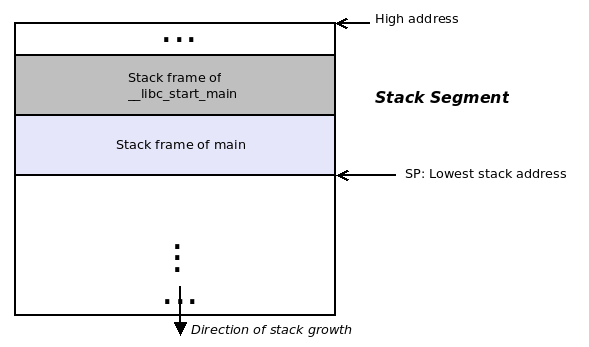
\includegraphics[width=.98\linewidth]{../figures/systemgrundlagen/stack.png}
	\caption{Stack segment}
	\cite{stack}
\end{wrapfigure}
The stack is a piece of memory where meta-data and local variables are saved when the \texttt{main()} function calls a routine/method. This memory segment is limited and doesn't allow an infinite number of data segments (also called stack frames) being stored in it. The stack uses assembly instruction like \texttt{pop} to delete a frame and \texttt{push} to add a frame. For consistency the stack will always pop the last element pushed. This is also known as \dq Last in First Out\dq{}\cite{stack}.\\
On UNIX systems we would create an attribute structure and pass the
desired options there. But because we don't use the unix's system function \texttt{pthread\_create()} we also
cannot use the attribute structure. Furthermore the standard library doesn't support such tweaks. 
This is very important if someone wants to use this for an ARM architecture, because he won't be
able to define a meaningful stack size. This doesn't pose any threats for many operating systems out
there, but for ARM, which has a limited stack size can be problematic. For windows this attribute
can be set using the \texttt{Create\_Thread()} function just like in unix using \texttt{pthread\_create()}.
\newpage
\section{Concurrency}
\label{ssec:concurrency}
Concurrency means that two or more things are happening simultaneously. This pehnomenon is happening
everyday almost everywhere we look. Even we as humans are capable of such thing, for example walking
and talking at the same time. In computer science concurrency means that more than one process can
be execuvted at the same time. Many systems have this ability, because most of them are
multiprocessor computers. Even some single core computers can handle concurrency to some extent.
One calculation unit can handle one task at a time, but it can quickly switch to another task if
necessary. This is why sometime even single core units give the impression of resolving jobs
simultaneously\cite[Chapter~1]{concurrency}. Although performant this method does not come without its flaws. When a cpu gets a new task, the resources of the old task (eg. local variable, meta data of the current task, etc.)will be replaced by those of the new job. This is also known as \dq Context Switching\dq{}.
The order of task switching will be explained in detail in chapter *scheduling*.\\ 
Nowadays many systems measure the concurrency of a system by its number of hardware threads. This
unit of measure tells us how many independet tasks can the processor handle.
\section{CPU Affinity}
The affinity of a CPU determines the number of processors that one process can use for its threads.
This library offers methods to restrict the number of CPUs off which a process can run on. This is
sometimes desirable because of the following reasons:
\begin{enumerate}
	\item Data invalidation: When a process starts, the user cannot tell from outside on which CPU
	that thread started. When a process finishes its time-slice, he has to give up its CPU for
	others to use it and it come back later, but it won't necessarily start on the same CPU as the
	last time. \footnote{This is a part of context switching, which was discussed in chapter \ref{ssec:concurrency}}. When this happens, entries in that CPU's cached must be replace or removed,
	which is known as \dq Cache invalidation\dq{}. This is not a flawless method and cache inconsistencies
	can appear.
	\item Emergency CPU: On real-time systems, where human lives are at risks, many developers will
	deliberately block some CPUs ( on a multicore machine) to use them when the system returns
	erros and needs to immediately execute safety protocols. Because the CPUs were blocked
	from being used on other processes, these remain free and so the execution of the safety procedure can start without any delay (eg. context switching).
	
\end{enumerate}

By default most systems allow each process to use all CPUs. If the user turns off half of the
CPUs of a given process and tries to create an additional workload with the library's methods for that process, he must keep in
mind that the workload will also be cut in half because the threads have less processors to work on.
\section{Priorities}
When it comes to the priority of a process there is a big difference between a UNIX system and a
windows machine. On Windows the priority is determined by the priority class of the process and the
its thread priority.\\
\subsection{Windows}
Based on the winAPI documentation\cite{priorityClasses}, the classes can have the following values:
\begin{enumerate}
	\item IDLE\_PRIORITY\_CLASS (0x00000040): This is the lowest priority, processes belonging to this class run only if the system is idle and can be preempted\footnote{If a process is preempted that means it stops executing and yields the cpu} by a process with a higher priority
	\item BELOW\_NORMAL\_PRIORITY\_CLASS(0x00004000): This class has a higher priority than an idle-classed process but a lower priority than a normal-classed process 
	\item NORMAL\_PRIORITY\_CLASS(0x00000080
	): This is the default class for all processes created by the user
	\item ABOVE\_NORMAL\_PRIORITY\_CLASS(0x00008000): This class has a higher priority than an normal-classed process but a lower priority than a high-classed process
	\item HIGH\_PRIORITY\_CLASS(0x00000080): This class is usually used for time critical jobs
	\item REALTIME\_PRIORITY\_CLASS(0x00000100): This is the class with the highest priority and is rarely used because it stop most of the tasks on the calling machine
\end{enumerate}
Each class can be preempted by a higher priority class besides the realtime-class. Classes categorize only processes, but not their created threads. For these the following values can be set:
\begin{enumerate}
	\item THREAD\_PRIORITY\_IDLE(-15)
	\item THREAD\_PRIORITY\_LOWEST(-2)
	\item THREAD\_PRIORITY\_BELOW\_NORMAL(-1)
	\item THREAD\_PRIORITY\_NORMAL(0)
	\item THREAD\_PRIORITY\_ABOVE\_NORMAL(1)
	\item THREAD\_PRIORITY\_HIGHEST(2)
	\item THREAD\_PRIORITY\_TIME\_CRITICAL(15)
\end{enumerate}
These are similar to the classes mentioned above and can be interpreted alike.\\
\subsection{Linux}
On Linux however, the priority of a process is harder to be determined. This value is composed out of two main components: the nice value of the process and its thread priority.
\subsubsection{Nice Values}
Nice values can range from 20 to
-19 with 20 being the nicest value and so the smallest priority and -19 being the worst value and so
the highest priority. For a better understanding one could think that a process is nice, when he doesn't need
the CPU and so it lets other threads to use it. In my research one thing was mentioned and that is a low nice value (hence a high priority) doesn't mean other processes won't get any CPU
time. The scheduler will make them more favorable, but other processes will also get their turn for the
CPU.
To change the nice value of a process, in this library, I am using
the calls \texttt{getpriority()} and \texttt{setpriority()} from the header \texttt{sys/resource.h}.\\
There is one
critical thing that the caller needs to know. In order to increase the nice value of the calling
process, the user can use the given methods of the library and additionally use the command
\texttt{sudo setcap cap\_sys\_nice=ep PATH/TO/EXECUTABLE} on the built binary (the command \texttt{setcap} can change the executable to
run as a privileged process, but only when called as root or with the keyword sudo), run it as root or build the executable
program as the root-user from the beginning. You need to do this extra step,
because by default any user-created processes are unprivileged.\\
Unprivileged processes can lower their own
priority, but are not allowed to increase it more than the value of the operation
\textit{20-RLIMIT\_NICE}. The RLIMIT\_NICE is resource on your UNIX machine and can be set/gotten with the methods \texttt{getrlimit()} and \texttt{setrlimit()} respectively. These functions takes as arguments an integer, which describes the resource we want to get or set (in this case RLIMIT\_NICE) and a \texttt{struct rlimit} pointer, which describes the priority of the given resource. The structure \texttt{rlimit} has two attributes: the \dq rlim\_cur\dq{}(also called the soft limit), that represent the current value of the process and the \dq rlim\_max\dq{}(also called the hard limit or ceiling), which tells one user the limit of which that process can be set to. On my testing system
RLIMIT\_NICE is set to 13 and the limits for processes compiled by my users are zero.
\begin{figure*}[!htb]
	\centering
	\subfigure[RLIMIT\_NICE code]{
		\label{RLIMIT_NICE_code}
		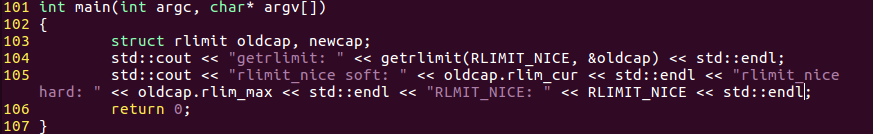
\includegraphics[width=0.9\textwidth]{../figures/systemgrundlagen/RLIMIT_NICE_code.png}}
	\subfigure[RLIMIT\_NICE output]{
		\label{RLIMIT_NICE_output}
		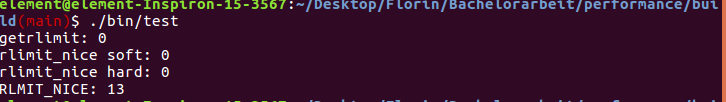
\includegraphics[width=0.9\textwidth]{../figures/systemgrundlagen/RLIMIT_NICE_output.png}}
	\caption{RLIMIT\_NICE} 
	\label{RLIMIT_NICE}
\end{figure*}
\\
Per default the process will have
the nice value of 0 and this value can be increased to the highest value allowed (19), but cannot be
decreased afterwards to a value lower than \textit{user\_nice\_value = 20-RLIMIT\_NICE}. A way of
increasing the nice value would be to increase the RLIMIT\_NICE value (also as root or with root-rights = sudo), which will allow a normal user to increase the value given until it reaches
\dq user\_nice\_value\dq{} or log in as root, use the library's functions, build the program and set the SUID as root.
\footnote{The SUID is a special bit that one can set and allows normal users to run the program as they
were root}\\
At last you could also modify the \dq/etc/security/limits.conf\dq{} file and set a new max nice value for a
certain user, but this is not the best solution, because that user would have the power to change
priorities not only for one program, but for all programs.
\subsubsection{Scheduling}
Unlike Windows, Linux has methods to change one's process and its threads scheduling policies.The default policy set on UNIX
is called "Round-Robin Timesharing" (SCHED\_OTHER). This allows jobs to be executed in a round robin fashion where
each process gets an equal time-slice of a CPU. There are more than one policy which can be set.
These are:
\begin{enumerate}
	\item SCHED\_OTHER
	\item SCHED\_BATCH
	\item SCHED\_IDLE
	\item SCHED\_FIFO
	\item SCHED\_RR
\end{enumerate}
The difference between SCHED\_RR and "Round Robin Timeshare"(SCHED\_OTHER) is that the realtime policy lets
us to coordinate the priorities for that schedueling policy's queue.\\
The differences are that BATCH schedules a process less
frequently, if the it gets the CPU very often and IDLE is the equivalent to a process with a nice value of 19
(very nice process <=> lowest value).
SCHED\_BATCH and SCHED\_IDLE are two normal prioritised policies, which differ from SCHED\_OTHER, but
not enough for me to focus too much on them.\\
You can get the current policy of your process by calling \texttt{int sched\_getscheduler(pid\_t pid)} from the \texttt{<sched.h>} header file. 
\\
Each of the policies mentioned above has a range of priorities levels, which can be get using the \texttt{sched\_get\_priority\_max(int policy)} and \texttt{sched\_get\_priority\_min(int policy)} methods found in \texttt{<sched.h>}.\footnote{These can be different depending on the calling xUNIX
machine}\\
On my Linux Notebook I have the following values:
\begin{figure*}[!htb]
	\centering
	\subfigure[sched\_prio\_range code]{
		\label{sched_prio_range_code}
		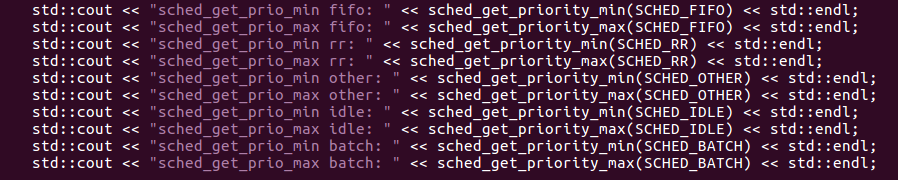
\includegraphics[width=0.9\textwidth]{../figures/sched_prio/sched_prio_range_source.png}}
	\subfigure[sched\_prio\_range output]{
		\label{sched_prio_range_output}
		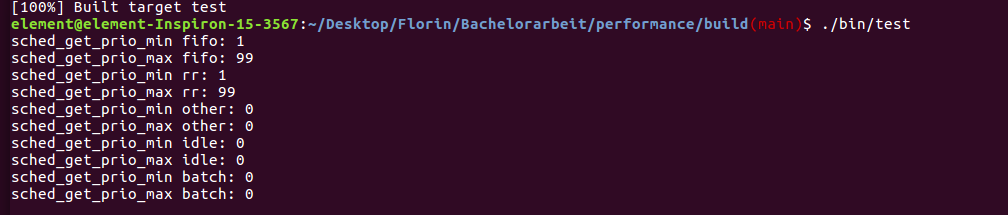
\includegraphics[width=0.9\textwidth]{../figures/sched_prio/sched_prio_range_output.png}}
	\caption{sched\_prio\_range} 
	\label{sched_prio_range}
\end{figure*}
You can only change the priority of real-time policies. hence when you set the policy of a thread to OTHER, IDLE or BATCH you can't change the priority of that process.\\
As you can observer only two of these have a \dq real\dq{} range.
SCHED\_RR and SCHED\_FIFO are characterized as real-time policies and have a higher priority than the
others. When two processes with SCHED\_RR and respectively SCHED\_FIFO have to share a CPU,
ironically the one that was placed first in that CPU's queue will get to run its job. Both of these
policies can lose access of their CPU, if they finish execution, yield\_sced() or a syscall is called
and a higher priority process preempts them (a process with a lower nice value appears in the queue
or the user changes the value himself). SCHED\_RR can also lose its access if the timeslice of
the job expires.

\section{Workload}
The definition for workload varies from field to field. In the IT-branch it is defined as a unit of measure for your CPU (mostly in \%). This tells the user how well his system can handle the number of current running processes. Most systems calculate their workload over a defined period of time. To understand this concept better, here is an example. Let's say a user starts a calculator program at time $\mathrm{t}_0$ = 0. The application will finish initializing a GUI at time $\mathrm{t}_{wait}$ = 2s and then an interactive visual window will appear, which will wait for the user to enter some equation.
After the equation was typed at $\mathrm{t}_{input}$ = 5s and the \dq Enter\dq{}-key was pressed, the application proceeds calculating and delivers the answer at $\mathrm{t}_{done}$ = 6s. So the CPU-time of the application is 3s(GUI initialization and calculation time). In order to get its workload the system has to divide this time by the time the system needed for the whole process and multiply it by one hundred to have the result as percentage:
\begin{equation}
	workload =  \frac{\mathrm{t}_{wait}+\mathrm{t}_{calc}}{6s}*100
\end{equation} 
A detailed explanation on how to get the values of these specific times will follow in Chapter (*Kapitelnr*).

\section{Synchronization}
When working with threads, the programmer cannot forget that these share the same stack, therefore they share the same variables. When two or more threads start their execution (eg. a simple addition), one cannot tell when will they perform what (if their priorities weren't tampered with).\\
There are two main operations threads can perform on a variable: \texttt{read()} and \texttt{write()}. Reading from a variable is not problematic, because its content will always stay the same, but writing to one is a whole different story. Let's take a look at the following code:
\begin{figure}[!htb]
	\centering
	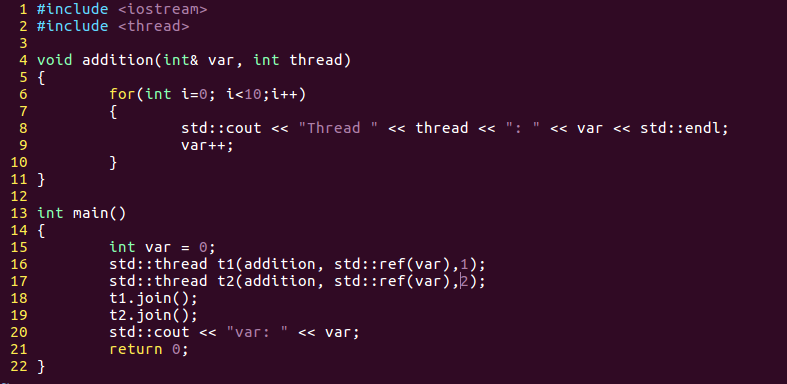
\includegraphics[width=0.5\textwidth]{../figures/systemgrundlagen/synchronizationExample.png}
\end{figure}
Here we create two threads with the sole purpose of adding a common variable. Most people would expect, because of the order of creation, for t1 to do his job and afterwards t2, but this is not the case.
\newpage
%\begin{figure}[!h]
%	\centering
%	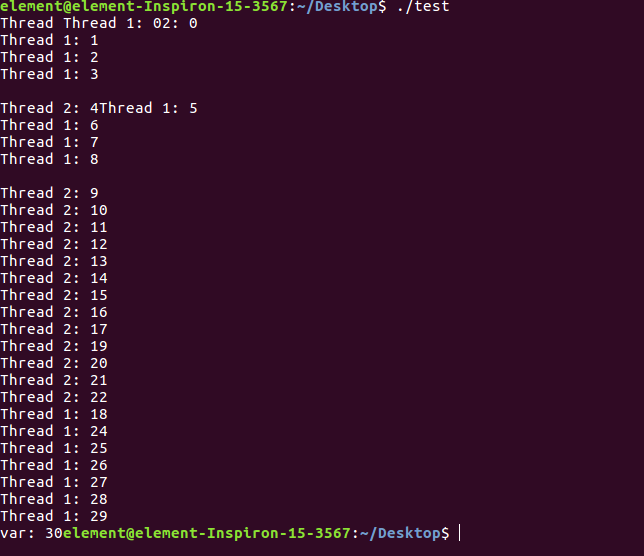
\includegraphics[width=0.5\textwidth]{../figures/systemgrundlagen/synchronizationExampleOutput.png}
%\end{figure}
\begin{wrapfigure}{1}{0.5\textwidth}
	\centering
	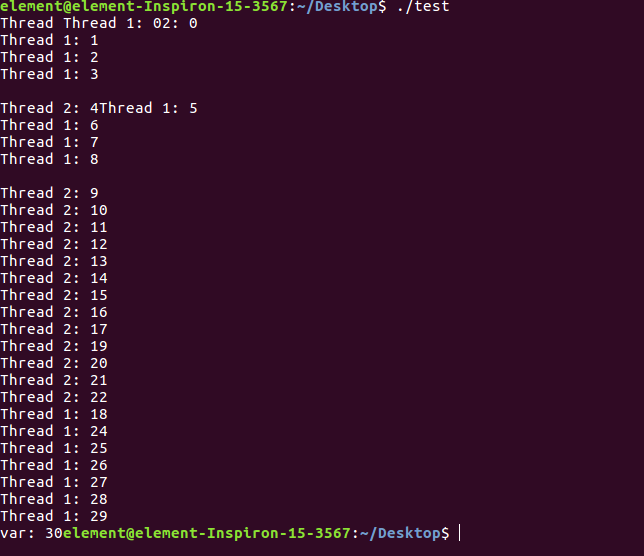
\includegraphics[width=.98\linewidth]{../figures/systemgrundlagen/synchronizationExampleOutput.png}
	\caption{Stack segment}
\end{wrapfigure}

As you can observe, these prints make no sense. The threads do not follow a sequentially pattern so the variable can be increased by \texttt{t1} for a time then by \texttt{t2} and for the rest of the remaining time by \texttt{t1} again.\\
Something that cannot be seen in the output would be the scenario when \texttt{t1} and \texttt{t2} try to access the variable and increment it at the same time. No one can accurately predict what the result would be (this is also known as \textit{ Unexpected behavior}). To resolve this problem in classic C people came up with the idea of a locking mechanism called \texttt{Mutex}.\\
\subsection{Mutex}
Mutexes are guards that can block other threads the access to variables inside a user-defined block of code (also known as \textit{scope}). These allow the thread that called \texttt{lock()} exclusive access to the variables inside that scope until the thread calls \texttt{unlock()}. If another thread tries to lock the mutex for himself while the mutex is being used, then it will land in a waiting state until that lock is released. This method requires a lot of concentration from the programmer and a good overview of all locking and release point\cite{concurrency}.\\
Fortunately the \textit{Standard C++ Library} implemented a new, more simplistic technology for threads to access common variable called \textit{Atomic Variables}.
\subsection{Atomic Variables}
Atomic variables can be seen as wrappers for primitive data types, like \texttt{bool}, \texttt{int}, \texttt{double}, \texttt{float}, etc., but also for defined structs like \texttt{uint32\_t}, \texttt{uintptr\_t} or \texttt{int\_fast32\_t}\\
Basic syntax of this wrapper is: \textit{atomic<data\_type/class>} or (if defined) \textit{atomic\_data\_type}, that will grant the calling thread exclusive access to a certain variable while reading from or writing to it.\\
To read from an atomic variable one could just use the \dq =\dq{}-operator or (preferred) the \texttt{atomic\_var.load()} method. Writing to an atomic variable should only be done by using the \texttt{atomic\_var.store()} method, because this way you can expect that no one else besides the calling thread is accessing that variable\cite{stdAtomic, atomicConference}.\\
The library comes with additional member functions to make certain sequences of reading and writing easier and specialized member function that define bitwise operations on a variable, but they go way too deep in complexity and understanding for me to focus too much on them. %Systemgrundlagen
\chapter{Library Overview}
This chapter will cover the library's build system and its main components, the system and workload components, as well as their logic.\\
The library has two main components. The first one is the workload, which can vary depending of the user's input. This will create a system specific amount of threads and make them run a simulation function. The number of threads will stay constant and the time for running the workload task will be set accordingly for each input.\\
The second components is the system. This comes with functions, which can easily change a thread's priority, a system's scheduling policy and deliver statistics of the user's computer.\\
Basic operations are implemented to work on most operating systems, but there are some exceptions because of the differences between OS implementations, which makes them independent from one another.
\section{Workload}
This part of the library is mainly a C++ class, that lets the user create a specific workload.
\begin{figure}[!htb]
	\centering
	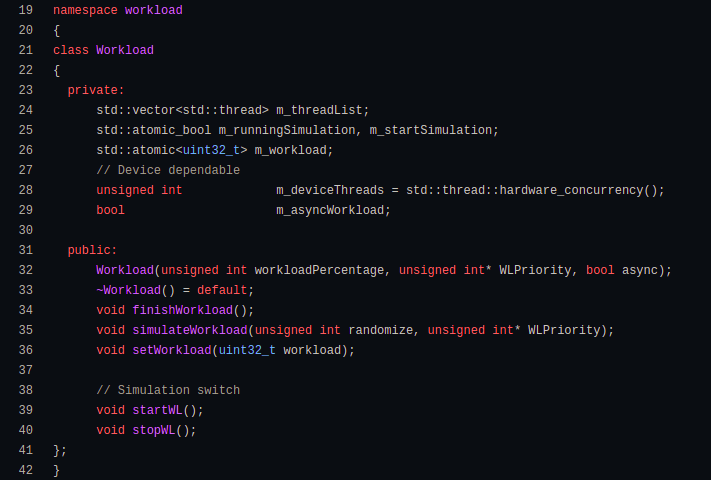
\includegraphics[width=0.5\textwidth]{../figures/libraryOverview/workloadClass.png}
	\caption{Thread's behavior without synchronization - Source code}
\end{figure}
\subsection{Attributes}
The class has six private Attributes:
\begin{enumerate}
	\item threadList: is a list of type vector that holds the current number of working threads after the initialization
	\item runningSimulation: is a flag that tells the user the status of his working threads. This will be set to true once at least one thread in \texttt{threadList} has started executing a routine
	\item startSimulation: is a switch that starts a simulation function (in our case \texttt{simulateWorkload()}). This is in order to synchronize threads and start them simultaneously
	\item workload: hold the current workload set by the user. This is meant for future implementations in order to let the user change workloads dynamically at runtime
	\item deviceThreads: is the number of threads the current machine can handle at the same time. This depends on the processor that the executable is running on therefore can differ on different device
	\item asyncWorkload: this is a flag for testing purposes in order to simulate a \dq real\dq{} workload. This will be explained in detail in *section*.
\end{enumerate}
The name start with \dq m\_\dq{} in order to tell the programmer that the variable is a member of the class. It makes it easier to read and informs the user about the variable at the same time, without the need to check the class's definition.

\subsection{Methods}
The class's methods are:
\begin{enumerate}
	\item \texttt{Workload()}: this is the class's constructor and takes three arguemnts:
	\begin{enumerate}
		\item workloadPercentage: given workload percentage, that the user wants to simulate
		\item WLPriority: this is a pointer to a OS-specific thread's priority. If this is set to \textit{NULL}, all threads will have the same (default) priority
		\item async: let	s the user to create a more \dq real\dq{} workload. This will be explained in detail in chapter***  
	\end{enumerate}
	The first thing the constructor checks when a new object is created is the validity of the passed workload. Next it sets the \textit{runningSimulation} and \textit{startSimulation} attributes to false for a synchronized start. Afterwards it measures the current workload for ten seconds (it can be less or more, but ten seconds is in my opinion a proper chunk of time) in order to warn the user for a possible system overload.
	At last, the workload's given percentage is stored in the attribute \textit{workload}, an output will inform the user about the number of threads that will be created and the loop creates the threads with the class's \texttt{simulateWorkload} method.\\
	\texttt{emplace\_back()} pushes the created threads into an \texttt{std::vector}. I opted for this method instead of \texttt{push\_back()} because the compiler doesn't have to create the thread temporarily and push it afterwards, but it uses the \texttt{std::move} mechanism where the object is moved directly after the creation. This way we spare ourselves some extra memory (which is a very important factor if this is used on an ARM architecture)
	\item \texttt{$\sim$Workload()}: this is the class's deconstructor. It is set to default and should be changed for future development
	\item \texttt{finishWorkload()}: this function iterates through the class's thread list, checks if these are joinable (in case some user used detach for some reason) and joins them. In case a thread cannot be joined the \textit{TID} will be printed to the console\newpage
	\item \texttt{simulateWorkload()}: this takes two arguments
	\begin{enumerate}
		\item randomize: is the index in the thread's construction loop
		\item WLPriority: is the priority passed in the constructor. If this is not \texttt{NULL}, the given priority will be set
	\end{enumerate}
	First the functions increases the priority of the calling thread to maximum, then it waits for all threads to be created. When that happens the attribute \texttt{startSimulation} will be set to true, this way we ensure a finer synchronisation between the threads, because reading from a variable and leaving the loop should take less time than the time gap between the thread's creation. Next, each thread sleeps for a couple of milliseconds, if \texttt{asyncWorkload} is set. This way each thread starts with a small delay so the library's workload will never be zero. One can imagine a sinus curve if the flag is set and a square wave function otherwise (as seen in Figure \ref*{workloadTimeDiagram}).
	\begin{figure*}[!htb]
		\centering
		\subfigure[\texttt{asyncWorkload} not set]{
			\label{syncWorkloadDiagram}
			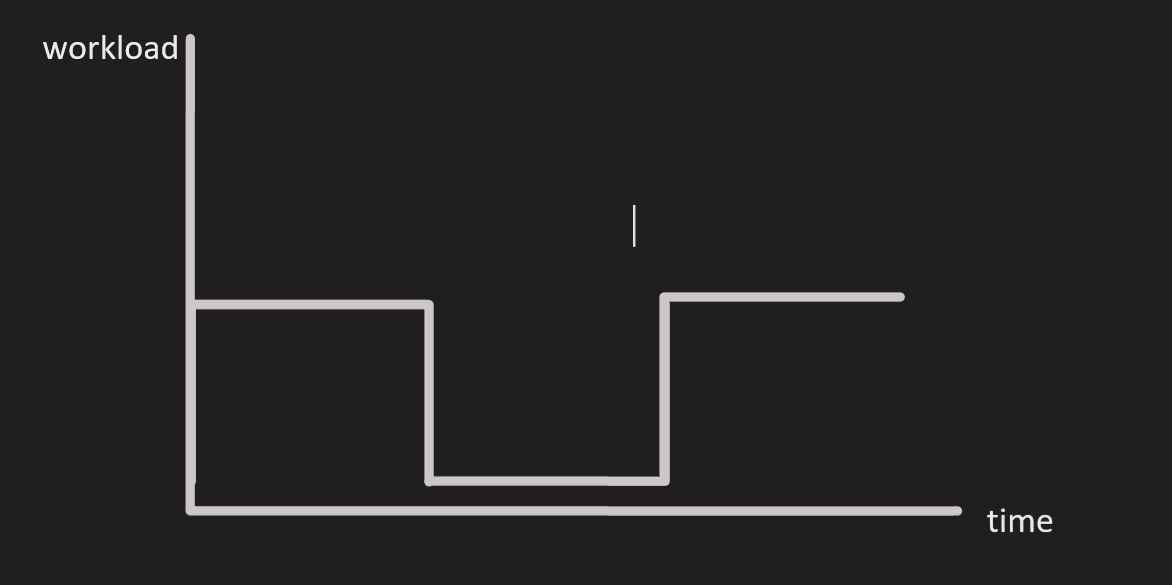
\includegraphics[width=0.7\textwidth]{../figures/libraryOverview/sync_workload.JPG}}
		\subfigure[\texttt{asyncWorkload} set]{
			\label{asyncWorkloadDiagram}
			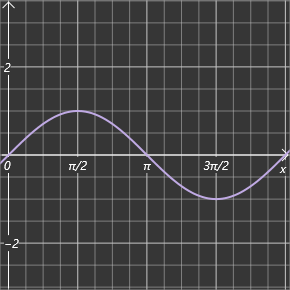
\includegraphics[width=0.4\textwidth]{../figures/libraryOverview/async_workload.png}}
		\caption{Workload Time Diagrams} 
		\label{workloadTimeDiagram}
	\end{figure*}
	Afterwards the actual workload loop will start. I decided to recalculate the sleep time based on the current workload here, in order to support future dynamically changing workload for the simulation. The frequency of the workload is hard coded to ($\frac{2*workload}{100}$)Hz,because a cycle of working and sleeping for a thread is half a second and the system measures the workload once a second so this highly depends on how often the library's system component makes its time measurements.	
	\item \texttt{setWorkload()}: this method's concept is to let the user dynamically change the thread's priority 
	\item \texttt{startWL()}: checks if all threads that needed to be created were saved in the thread list. If this is the case it sets \texttt{simulationStart} and \texttt{runningSimulation} to \textit{true}
	\item \texttt{stopWL()}: sets \texttt{runningSimulation} to \textit{false}. It makes sense to call this method before \texttt{finishWorkload()}, in order to properly stop all workload threads
\end{enumerate}
\section{System}
This part of the library mainly contains methods to modify a thread's or process priority, the number of CPUs the a process can run on (see the cpu's affinity \ref{ssec:cpu_affinity} and the scheduler's policy \ref{ssec:sched_policies}).
\subsection{Defines}
\begin{enumerate}
	\item STR\_ERR: macro returned by a function if it failed
	\item IDLE\_TIME: macro that represents idle time of the system
	\item USER\_TIME: macro that represents user time of the system
	\item KERNEL\_TIME: macro that represents kernel time of the system
	\item schedPrioList: vector containing scheduler classes for a WINDOWS machine in ascending order(mentioned in \ref*{winPrioClass})
	\item threadPrioList: vector containing thread priorities for a WINDOWS machine in ascending order(see \ref*{winPrioClass})
	\item sched\_attr: struct containing thread's attributes for a LINUX machine
\end{enumerate}
\subsection{Methods}
\label{system-methods}
\begin{enumerate}
	\item Windows:
	\begin{enumerate}
		\item mergeFILETIME(): takes a FILETIME structure as argument, merges the two 32-Bits attributes of the struct into a uint64\_t variable and returns it
		\item setCPUAvailability():
		\begin{enumerate}
			\item proc: is a windows identification struct for processes of type \texttt{HANDLE}
			\item mask: a 64-Bit value representing the cpu affinity for most computers out there. Each bit represents a cpu. If a bit is set to 1,that means the process can run on the CPU corresponding to that bit.
		\end{enumerate}
		\item increaseSchedClass():this method gets the current scheduler class and checks if it is already set to the maximum value allowed. In that case it will not do anything, throw and error and return 1. Otherwise it will get the index of the current class in the \texttt{schedPrioList}, increase the index by one and set it accordingly. This allows the user to test its program step by step without knowing the actual values in the list. If the user wants to set a certain value for his thread, he can simply use the \textit{winAPI} functions.
		\item decreaseSchedClass(): does almost the same as \texttt{increaseSchedClass()}, but instead of increasing the scheduler class's priority, it decreases it
	\end{enumerate}
	\item Linux/Unix:
	\begin{enumerate}
		\item readCPUTime(): this functions takes an argument of type integer and reads data about the CPU specified by the given number. The data read comes from the \dq/proc/stat\dq{} file. As described in the manual page, the proc filesystem provides informations about the kernel structure or in other words about all processes on the calling system. The \dq/proc/stat\dq{} file contains statistics about the system.\\
		This component uses only the first line and the lines which begin with the name \textit{cpuN}, where \textit{N} stands for the CPU specified by the argument passed to this function. Each line that contains statistics about the CPU has the following pattern\cite{linux-man-proc}:\\\\\vspace{1cm}
		\begin{tabular}[h!]{ |c|c|c|c|c|c|c|c|c|c|c| }
				\hline
				name & user & nice & system & idle & iowait & irq & softirq & steal & guest & guest\_niced\\
				\hline
		\end{tabular}\\
		The most important statistics for the library are\cite{linux-man-proc}:
		\begin{enumerate}
			\item name: is either cpu or cpuN, where cpu stands for the whole system and cpuN for a cpu specified by N, where N$\in$ [0;max\_number\_of\_CPUs]
			\item user: is the time spent in user mode
			\item nice: is the time spent in user mode with low nice values
			\item system: is the time spent in system mode
			\item idle: is the time spent for idle tasks
		\end{enumerate}
			If the function is successful, it always returns an \texttt{std::string} containing the line specified by the passed argument, else it return the macro \texttt{STR\_ERR}.
		\item returnData(): this function takes an integer as its argument specifying the cpu that we want data from. If the integer is zero, the function returns data from the whole system, one for the first cpu, two for the second cpu and so on. If the given integer is higher than the value returned by \texttt{std::thread::hardware\_concurrency()} or lower than zero the function will fail and throw an exception, else the argument will be passed to the \texttt{readData()} method, parse the string returned by it and return the data as an \texttt{std::vector} containing \texttt{uint64\_t} values.
		\item printPolicy(): this is a utility function that takes an integer as the argument and prints the policy corresponding to it. Possible values are for the arguments are specified in \ref{ssec:sched_policies}.
		\item changedPolicy(): this functions takes two integer as its arguments:
		\begin{enumerate}
			\item policy(int): new policy that should be set
			\item pid(int): the process's \textit{PID}. If this is zero this function will change the policy of the calling process
		\end{enumerate}
		First this function uses system calls, \texttt{SYS\_sched\_getattr} to get the current \texttt{sched\_attr struct} specified in the linux man pages and \texttt{SYS\_sched\_setattr} to set the new one for the given process specified by the passed arguemnts.\cite{linux-man-set/getattribute}
		\item decreaseProcessNiceValue(): this method takes an integer as its argument specifying the pid and is similar to \texttt{decreaseSchedClass()}, but instead of checking a local vector list, it uses \texttt{getpriority()} with \texttt{PRIO\_PROCESS} and \texttt{pid} to get the current nice value, saves it temporarily and decreases/increments it by one. Then it uses \texttt{setpriority()} to set the new value with the same arguments passed to \texttt{getpriority()}. If the nice value reaches 20, the function will throw an exception. The method will fail only if \texttt{set/getpriority} fails.
		\item increaseProcessNiceValues: this method does the same as its former mentioned function, but instead of decreasing/incrementing the value this method increases/decrements it.
	\end{enumerate}
	\item NON-OS-Specific:\\
	NON-OS-Specific functions refrain to methods that either don't depend on any of the OS-Specific libraries such as the UNIX header files and the winAPI or they give the impression of identical behaviour, while in reality each case is manged with a lock-guard. 
	\begin{enumerate}
		\item getCPUTimes(): this function takes the following arguments
		\begin{enumerate}
			\item kernel(uint64\_t reference\footnote{A reference is like a pointer but the variable passed cannot be \textit{NULL}}): kernel time -> time the CPU spent for more \dq privileged\dq{} methods like system calls or interrupts
			\item user(uint64\_t reference): user time -> this refers to any other methods for example a simple loop written by the user
			\item idle(uint64\_t reference): idle time -> this time shows how long the system has been idle 
		\end{enumerate}
		This function gets the three times specified by the arguments and writes them in the passed references for further usage.\\
		On Linux it uses the \texttt{returnData()} method with zero as its argument and it saves the first four entries of the returned vector. The zeroth and first entry sum up the user time, the second is the kernel time and the third is the idle time.\\
		On Windows it first creates three \texttt{FILETIME} variables and uses \texttt{GetSystemTimes()} to get the three specified times. If \texttt{GetSystemTimes()} fails, an exception will be thrown and the function will return one, otherwise it will call \texttt{mergeFILETIME()} (because a FILETIME variable is a struct that contains two 32-bit attributes and one needs to concatenate the lower bits to the upper bits to get the real time as a 64-bit variable).
		\item getProcessTimes(): this function takes two uint64\_t references as its arguments and writes the user and kernel times in them. The methods used to get these times do not deliver the idle time (logically thinking there is no user case when this might be important).\\
		On Linux the function calls the \texttt{times()} method specified by the \texttt{<sys/times.h>} header file. This writes the required times of the calling process in two attributes of type \texttt{clock\_t} called \textit{tms\_utime} and \textit{tms\_stime} which belong to a  data type called \texttt{struct tms} (this also contains the kernel and user time of any process children created by the current process, but these are irrelevant for this implementation).\\
		On Windows it uses \texttt{GetProcessTimes()} to get the times similar to \texttt{getCPUTimes()}. It uses \texttt{GetCurrentProcess()} to specify the current process. \texttt{GetProcessTimes()} also delivers the creation and exit time, these are irrelevant for this implementation. If \texttt{GetProcessTimes()} fails the function will throw an exception and will return one.
		\item convertTime(): this is a utility method and takes a uint64\_t as its argument representing the time. \\
		On Linux \texttt{sysconf(\_SC\_CLK\_TCK)} is called, which returns the system's clock ticks per second value. If this is fails an exception is thrown and the functions returns minus one, otherwise it return the seeked time in milliseconds.\\
		On Windows it returns the given argument multiplied by 0.1, which also represents the time in milliseconds.
		\item getSpecificCPUTime(): the method is more utility based and similar to \texttt{getCPUTimes()}, but instead of writing its times into the passed arguments, it returns only one time described by the given parameter. Its type is an integer and describes which CPU time should be returned as a uint64\_t value. Possible arguments are \texttt{IDLE\_TIME}, \texttt{USER\_TIME} and \texttt{KERNEL\_TIME}, which are defined in \texttt{system/system.hpp} file and extend to zero, one and two respectively.
		\item increase-/decreaseThreadPrio(): is similar to \texttt{increase-/decreaseProcessNiceValue()} or \texttt{increase-/decreaseSchedClass()}.
		On Linux the method takes an integer as parameter called \textit{id}, which it gets the current TID (if \textit{id} is zero, which is set by default) priority or the priority specified by \textit{id} with the help of \texttt{sched\_getsched()}. Afterwards it initializes a \textit{sched\_attr} struct, increases or decreases the priority (throws an error if the maximal or minimal priority is reached) and sets the priority through a system call\footnote{Using the system call is preferred, because it supports future development of the function for tempering with more thread's attributes and not only the their priority}. \\
		On Windows it does the same. The only difference is in the parameter and the functions called to get and set the thread's priority. Here the \texttt{GetThreadPriority()} and \texttt{SetThreadPriority()} are used which expects a \textit{HANDLE} type as their arguments. That's why we also pass a \textit{HANDLE} to this function instead on an \textit{integer} as TID.    
		\item calculateSystemLoad(): the function calculates and returns the system's current workload as a double value\footnote{This is mainly used in the workload class to tell the user the system's current workload and not overload the system}. It takes an integer as its arguments, which specifies the duration of the check.
		On Linux it adds the kernel time to the user time, divides the sum to the addition of kernel, idle and system time and multiply the result with 100 to get a workload as a percentage. 
		\begin{equation}
		workload =  \frac{\mathrm{t}_{user}+\mathrm{t}_{kernel}}{\mathrm{t}_{user}+\mathrm{t}_{kernel}+\mathrm{t}_{idle}}*100
		\end{equation}\\
		On Windows however kernel time also contains the idle time of the system (as specified in the winAPI documentation), so in order to get a meaningful and correct result we have to subtract idle time from kernel time.
		\begin{equation}
		workload =  \frac{\mathrm{t}_{kernel}-\mathrm{t}_{idle}+\mathrm{t}_{user}}{\mathrm{t}_{user}+\mathrm{t}_{kernel}}*100
		\end{equation}\\
		\item calculateAndShowLoad(): this functions takes three parameters:
		\begin{enumerate}
			\item duration: the duration of the check while the load simulation is active
			\item processWLList: a \textit{vector} that contains entries with the process's workload in one seconds intervals. So the number of entries is also defined by the duration of the check
			\item systenWLList: also a \textit{vector}, which contains the system's workloads during the check. It size also depends on the duration of the check 
		\end{enumerate}
		It also calculates the system's and process's workloads similar to the latter. But instead of just printing it to the screen it saves the values into lists (\textit{std::vectors}) used later for writing logging files. Before terminating it also determines the time which the system was not idle using the \texttt{convertTime()} and \texttt{getSpecficCPUTime()}
		\item writeOverallStats(): this operations takes two arguments:\\
		1) \textit{stat}, which represents the number of the statistic that will be written to the log file 
		2) \textit{statName}, a string representing the name of the stat
		After calling this functions, it will try to create and open a \textit{comma separated file}(CSV) named \dq \textit{overall\_stats.csv}\dq{}. If this fails an exception will be thrown and the function returns -1. Otherwise it will write the given stat with the given name string passed by \textit{statName} and close the file.
		\item wirteRuntimeStats(): similar to the latter, this functions writes all statistics given by its first argument with the name passed into the second argument to a CSV file. If the CSV file could be successfully created and opened, it will write the statistics and close if afterwards. Otherwise the method will throw an exception and return -1.
	\end{enumerate}
\end{enumerate}
\section{Build System - CMAKE}
As described in \ref{objective} the goal of this library is to create methods supporting the two big operating systems in the industry: Linux and Windows. In order to do that the library comes with additional support for projects that use CMake for their build system. When calling the \textit{cmake} command on the main \textit{CMakeLists.txt}, the system will generate different files depending on the calling OS. When called on Linux, it will generate \textit{Make} files that can be used with the make mechanism that comes with most (almost all) \textit{UNIX} distributions to build the files specified in \textit{CMakeLists.txt} of each directory. When called on windows .... .
We can use the CMake syntax to either link the components to the library statically or dynamically\footnote{Static Library means that the linked libraries will be part of the executable, while the code from a Dynamically Linked Library will be linked at runtime, thus resulting in a much smaller sized executable. A good hint for the user when trying to link this library}. 
\subsection{Implementation}
As already mentioned, when using \textit{CMake} each directory needs a \textit{CMakeLists.txt}. The main file is the most important file, because it sets the requirements for the whole project.\\
The first requirement for this project is the minimum cmake version, which is set from 3.12 to 3.21. This way it supports even older version(if the user didn't bother updating the program). Then we set a failing criteria, for the user to know that the library doesn't support older versions. Afterwards we set some CMake standard variables to make the user have at least C++17 enabled. This is done for two main reasons: \\
First, the library uses newer elements for its components, therefore older versions won't be compatible and so errors will occur.\\
Second, the library should encourage the users to start implementing modern and up-to-date standards (in my opinion C++17 is not even a new standard, considering)
After that the library prints a message to tell the user what operating system was recognized by CMake and then we define the name of the project, the version, description and its programming language.\\
Finally we tell CMake which directories contain the code for our project by adding them to the include search path and linking the targets that are defined in those directories to the main executable target created in the \textit{CMakeLists.txt} that can be found in the source subdirectory.\textsl{}
%% Beispiele.tex
%%

\chapter{Beispiele}
\label{ch:Beispiele}
%% ==============================
Bla fasel\ldots

Beispiele

\section{Zitieren}
Quellen\cite{li00,jackson91,lakhina04a,netflow,rfc2386} 
nicht vergessen. Dazu verwendet ihr bibtex.

%% ==============================
\section{Bild einf�gen}
%% ==============================

\subsection{Ein Bild skaliert}

\begin{figure}[htbp]%Positionierung vorzugsweise an dieser Stelle. Falls nicht m�glich oben positionieren. Falls das auch nicht geht unten.
	\centering
		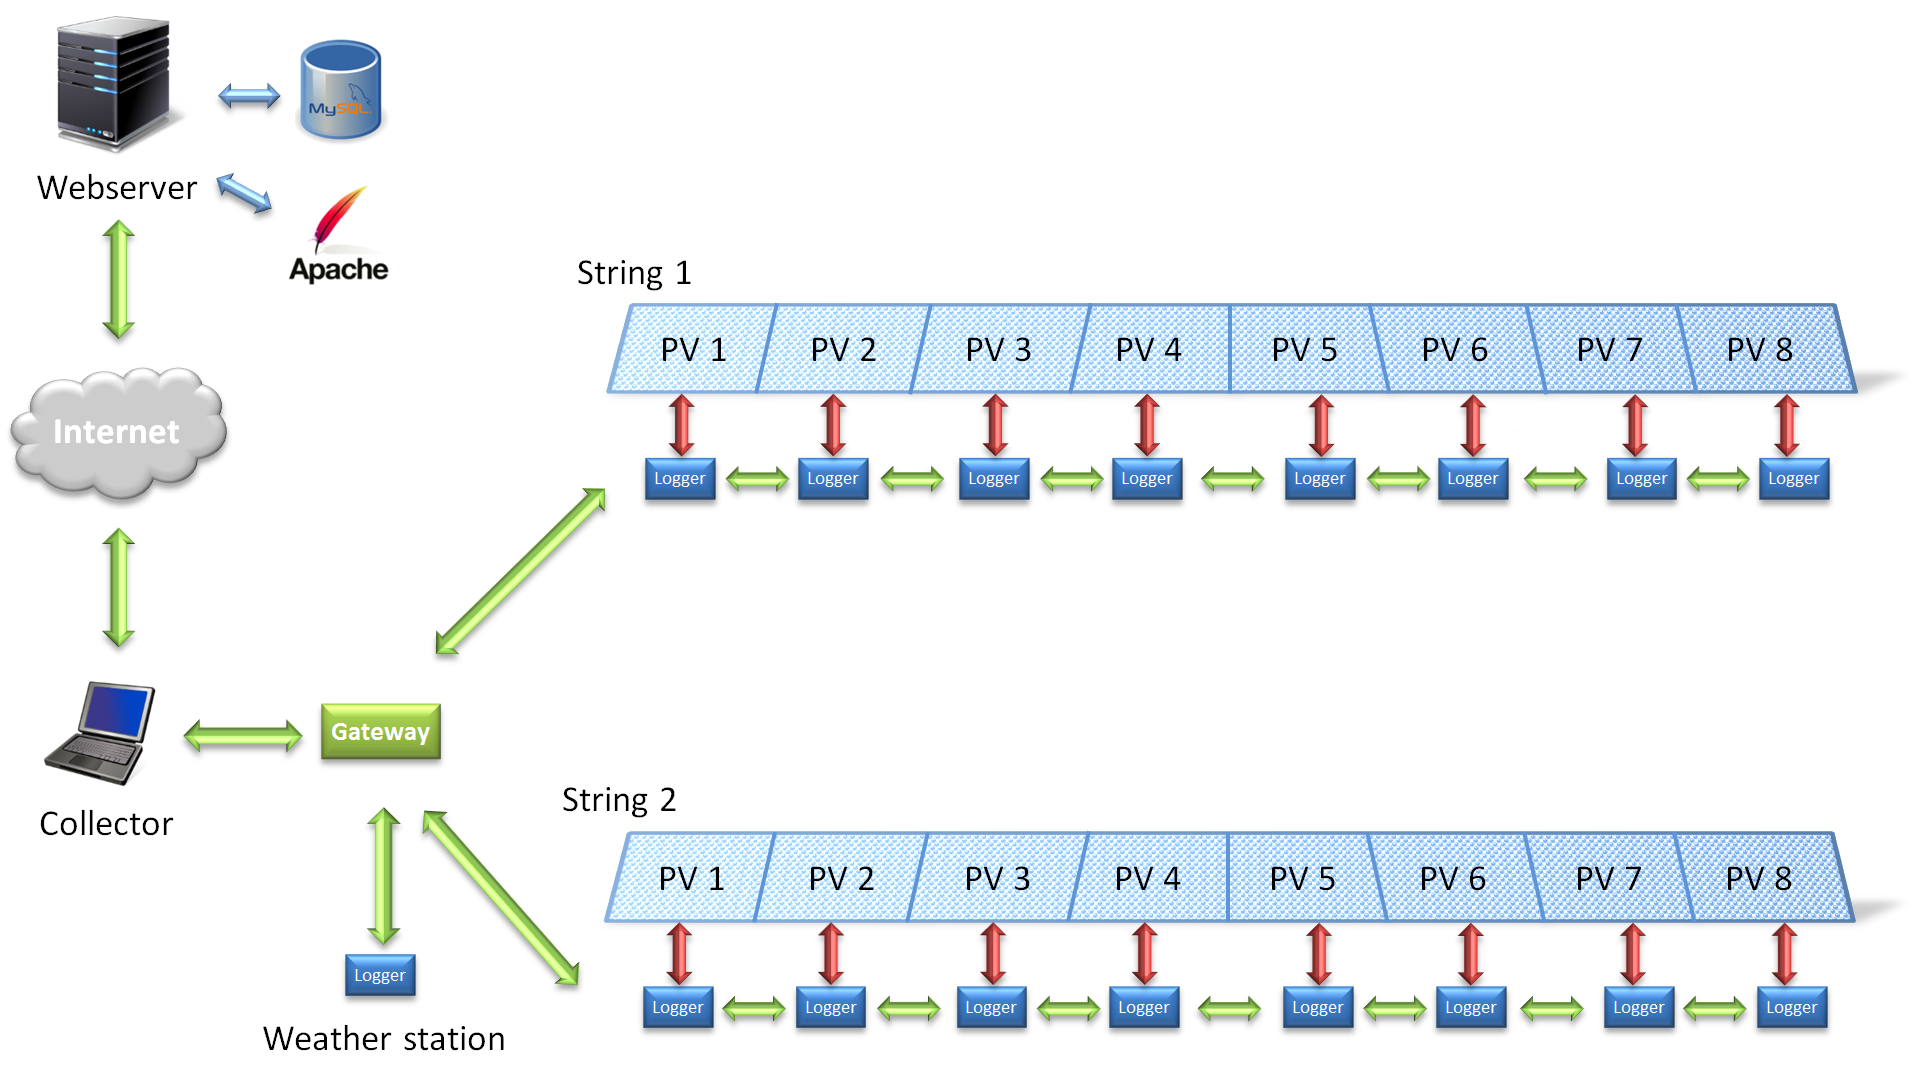
\includegraphics[width=0.80\textwidth]{../figures/large1.png}
	\caption{Beschriftungstext}
	\label{fig:large1}
\end{figure}

\subsection{Zwei Bilder nebeneinander oder untereinander}
%%%%%%%%%%%%%%%%%%%%%%%%%%%%%%%
\begin{figure*}[!htb]
	\centering
	\subfigure[Beschriftung Bild links]{
	  \label{fig:small1}
		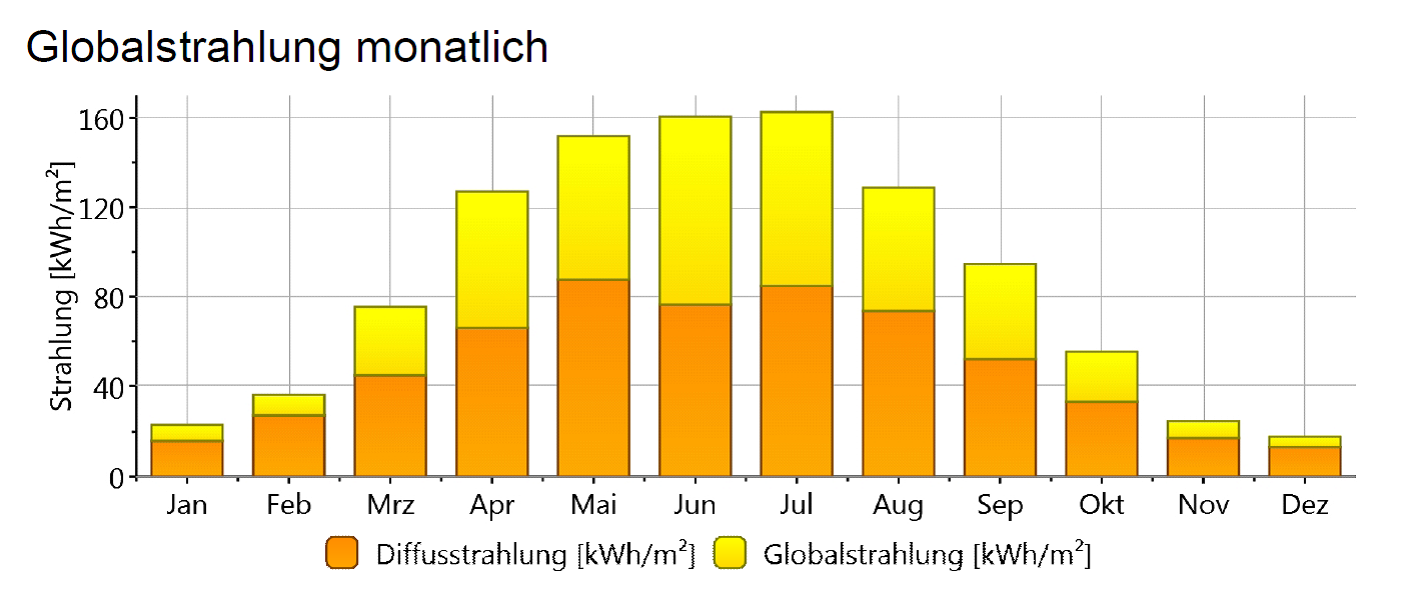
\includegraphics[angle=0,width=0.68\textwidth]{../figures/small1.png}}
	\subfigure[Beschriftung Bild rechts]{
	  \label{fig:small2}
		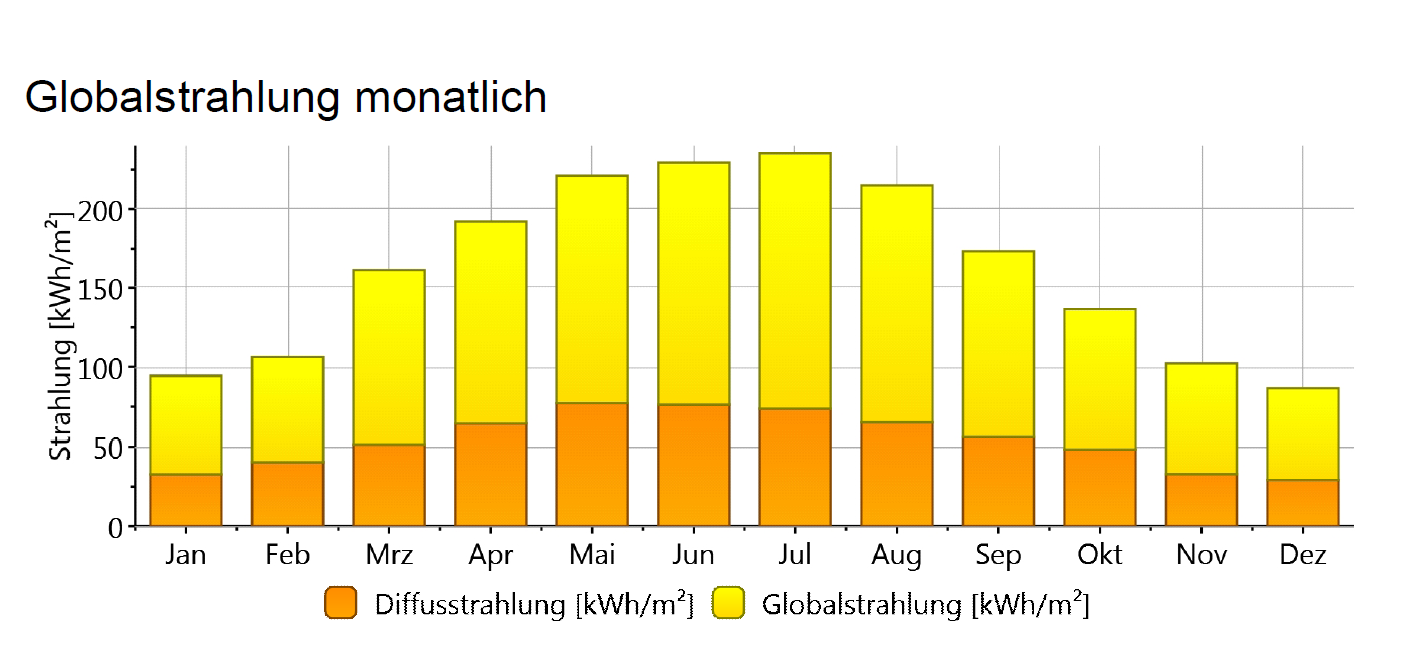
\includegraphics[angle=0,width=0.68\textwidth]{../figures/small2.png}}
 	\caption{Beschriftung beide Bilder} 
	\label{fig:beidebilder}
\end{figure*}
%%%%%%%%%%%%%%%%%%%%%%%%%%%%%%%


%% ==============================
\section{Tabellen}
%% ==============================
\begin{table}[htbp]
	\centering
		\begin{tabular}{|l|L{3.3 cm}|L{6.1 cm}|}
			\hline
			Firma								&			Produkte / L�sungen											&		WEB\\
			\hline
			Concentrix (Soitec)	&	Module mit Konzentratoren (Fresnel-Linsen)	&	http://www.soitec.com \\
			\hline
			Isofoton						&	Module mit Konzentratoren (Fresnel-Linsen)	&	http://www.isofoton.com \\
			\hline
			Semprius						& Module mit Konzentratoren (Fresnel-Linsen)	& http://www.semprius.com \\ 
			\hline
			\hline
			Azur Space					& Mehrfach Junction Zellenhersteller					& http://www.azurspace.com \\
			\hline
			Cyrium Technologies	& Mehrfach Junction Zellenhersteller					& \small{http://www.cyriumtechnologies.com} \\
			\hline
			Emcore							& Mehrfach Junction Zellenhersteller					& http://www.emcore.com \\
			\hline
		\end{tabular}
	\caption{Hersteller von CPV-Produkten}
	\label{tab:Hersteller}
\end{table}

\begin{table}[htb]
		\centering
		%\renewcommand{\arraystretch}{1.03}
		\caption{Single-hop Scenario - Traffic Pattern \label{t:traffic}}
			
		\begin{tabular}{l@{~}l@{\,\,}l@{\,\,}l} \hline \rule{-2pt}{12pt}
			Pattern& Parameter & Distribution & Range/Values  \rule{0pt}{12pt} \\ \hline \rule{-2pt}{12pt}  
      \textbf{Burst}      
      & Burst IAT         & uniform  & [9.9; 10.1] s\\ 
      & Packets per Burst & constant & 100\\
      & Packet IAT        & constant & 0.02 s\\
      & Packet Size       & constant & 1024 bit\\
      & \# Sources & -        & 2\\
			& Offset						& uniform  & [0; 1] s\\ 
      \hline      \hline\rule{-2pt}{12pt} 
      \textbf{Single}     & Packet IAT        & uniform  & [0.9; 1.1] s\\
      & Packet Size       & constant & 1024 bit\\
      & \# Sources & -        & [10;20;30;40;50;\\
      & & & 60;70;80;90;100]\\
			& Offset						& uniform  & [0; 1] s\\ 
      \hline
    \end{tabular}
\end{table}   % Beispiele
%% analyse.tex
%%

\chapter{Analyse}
\label{ch:Analyse}
%% ==============================
Bla fasel\ldots

%% ==============================
\section{Abschnitt 1}
%% ==============================
\label{ch:Analyse:sec:Abschnitt1}

Bla fasel\ldots

%% ==============================
\section{Abschnitt 2}
%% ==============================
\label{ch:Analyse:sec:Abschnitt2}
Bla fasel\ldots
\subsection{Unterabschnitt}
Bla fasel\ldots
\subsubsection{Unter-Unterabschnitt}

     % Analyse



%% ++++++++++++++++++++++++++++++++++++++++++
%% Anhang
%% ++++++++++++++++++++++++++++++++++++++++++

%\appendix
%\include{anhang_a}
%\include{anhang_b}

\ifnotonesideelse{\cleardoublepage}{}

%% ++++++++++++++++++++++++++++++++++++++++++
%% Literatur
%% ++++++++++++++++++++++++++++++++++++++++++
\addcontentsline{toc}{chapter}{\bibname}
%  mit dem Befehl \nocite werden auch nicht zitierte Referenzen abgedruckt 
% (normalerweise nicht erwünscht)
% \nocite{*}
\bibliographystyle{unsrt}
%Einbinden Bibtexdatei - Direkt aus JabRef generiert
\bibliography{literatur}
%\bibliography{links}
%% ++++++++++++++++++++++++++++++++++++++++++
%% Index (optional)
%% ++++++++++++++++++++++++++++++++++++++++++
%\ifnotdraft{
%\addcontentsline{toc}{chapter}{Index}
%\printindex            % Index, Stichwortverzeichnis
%}
\listoffigures
\end{document}
